\section{Introduction: PIT \& beyond}

Algebraic circuits are natural algebraic analog of boolean circuits, with the logical operations being replaced by $+$ and $\times$ operations over the underlying field. The study of algebraic circuits comprise the large study of algebraic complexity, mainly pioneered (and formalized) by Valiant \cite{valiant1979completeness}. A central problem in algebraic complexity is an algorithmic design problem, known as Polynomial Identity Testing (PIT): given an algebraic circuit $\calC$ over a field $\F$ and input variables $x_1,\hdots,x_n$, determine whether $\calC$ computes the identically zero polynomial. PIT has found numerous applications and connections to other algorithmic problems. Among the examples are algorithms for finding perfect matchings in graphs \cite{lovasz1979determinants, DBLP:journals/combinatorica/MulmuleyVV87,fenner2019bipartite}, primality testing \cite{agrawal2004primes}, polynomial factoring \cite{kopparty2014equivalence,dutta2018discovering}, polynomial equivalence \cite{dvir2014testing}, reconstruction algorithms \cite{klivans2006learning,shpilka2009interpolation,karnin2009reconstruction} and the existence of algebraic natural proofs \cite{chatterjee2020existence,kumar2020if}. Moreover, efficient design of PIT algorithms is intrinsically connected to proving strong lower bounds \cite{heintz1980testing,agrawal2005proving,kabanets2004derandomizing,dvir2010hardness,forbes2018succinct,chou2018hardness,dutta_et_al:LIPIcs.ITCS.2021.23}. Interestingly, PIT also emerges in many fundamental results in complexity theory such as $\IP=\PSPACE$ \cite{shamir1992ip,lund1992algebraic}, the PCP theorem \cite{arora1998proof,arora1998probabilistic}, and the overarching Geometric Complexity Theory (GCT) program towards $\P\ne\NP$ \cite{mulmuley2012gct,mulmuley2012geometric, grochow2015unifying,joshua16boundaries}. 

There are broadly two settings in which the PIT question can be framed. In the \emph{whitebox} setup, we are allowed to look inside the wirings of the circuit, while in the \emph{blackbox} setting we can only evaluate the circuit at some points from the given domain. There is a very simple randomized algorithm for this problem - evaluate the polynomial at a random point from a large enough domain. With very high probability, a nonzero polynomial will have a nonzero evaluation; this is famously known as the Polynomial Identity Lemma \cite{ore1922hohere,DL78,Zip79,schwartz1980fast}. It has been a
long standing open question to derandomize this algorithm.

For many years, blackbox identity tests were only known for depth-2 circuits which compute sparse polynomials \cite{ben1988deterministic,klivans2001randomness}. In a surprising result, Agrawal and Vinay \cite{agrawal2008arithmetic} showed that a complete derandomization of blackbox identity testing for just depth-4 algebraic circuits ($\SPSP{}{}{}$) already implies a near complete derandomization for the general PIT problem. More recent depth reduction results \cite{koiran2012arithmetic,gupta2013arithmetic}, and the bootstrapping phenomenon \cite{Agrawal8107,kumar2019near,DBLP:conf/focs/Guo0SS19,DBLP:conf/coco/000320} show that even PIT
for very restricted classes of depth-$4$  circuits (\emph{even} depth-$3$) would have very
interesting consequences for PIT of general circuits. These results make the identity testing regime for depth-$4$ circuits, a very meaningful pursuit.

\emph{Three PITs in one-shot.} Following the same spirit, here we solve three important (and open) PIT questions. We give the first deterministic polynomial-time whitebox PIT algorithm for the bounded sum of product of sum of univariates circuits \cite[Open Prob.~2]{saha2013case}. Further, we give a quasipolynomial-time blackbox algorithm for the same class of circuits. These circuits are denoted by $\SPSU{[k]}{}{}$ and compute polynomials of the form $\Sigma_{i \in [k]} \Pi_{j} \left(g_{ij1}(x_1)+ \cdots +g_{ijn}(x_n)\right)$.
\begin{quote}
    \itshape 
    Whitebox and Blackbox PIT for the $\SPSU{[k]}{}{}$ circuits is in polynomial and quasi-polynomial time respectively.
\end{quote}
%
A similar technique also gives a quasi-polynomial time blackbox PIT algorithm for the bounded sum of product of bounded degree sparse polynomials circuits. They are denoted by $\SPSP{[k]}{}{[\delta]}$ (where $k$ and $\delta$ can be up to \(\poly(\log(s))\), where \(s\) is the circuit size). 
\begin{quote}
    \itshape
    Blackbox PIT for the $\SPSP{[k]}{}{[\delta]}$ circuits is in quasi-polynomial time.
\end{quote}
%
$\SPSP{[k]}{}{[\delta]}$ circuits compute polynomials which are of the form $\Sigma_{i \in [k]} \Pi_{j} g_{ij}(\x)$, where $\pdeg(g_{ij}) \le \delta$. Even $\delta=2$ was a challenging open problem \cite[Open Problem~2]{DBLP:conf/coco/0001S16a}. The model has gained a lot of interest in the past few years and has generated many important results \cite{peleg2020generalized,peleg2020polynomial,GOS22,OS22}.

\vspace*{1em}
\subsection{Main results: An analytic detour to three PITs}
Though some attempts have been made to solve PIT for $\SPSU{[k]}{}{}$, an efficient PIT for $k \ge 3$  \emph{even} in the whitebox settings remains open, see \cite[Open Prob.~2]{saha2013case}. Our first result addresses this problem and designs a polynomial time algorithm (Ref. Algorithm \ref{algo:whitebox-algo}). In our pursuit we discover an analytic and non-ideal based new technique which we refer as $\mathsf{DiDI}$. Throughout the paper, we will work with $\F=\Q$, though all the results hold for field of large characteristic. 

\begin{theorem}[Whitebox $\SPSU{[k]}{}{}$ PIT] \label{thm:thm1}
There is a deterministic, whitebox $s^{O(k\,7^k)}$-time PIT algorithm for $\SPSU{[k]}{}{}$ circuits of size $s$, over $\F[\x]$.
\end{theorem}

\begin{remark*} ~ 
    \begin{enumerate}
        \item Case $k \le 2$ can be solved by invoking \cite[Theorem 5.2]{saha2013case}; but $k \ge3$ was open.
        \item Our technique \emph{necessarily} blows up the exponent exponentially in $k$. In particular, it would be interesting to design an efficient time algorithm when $k=\Theta(\log s)$.
        \item It is not clear if the current technique gives PIT for $\Sigma^{[k]}\Pi\Sigma\mathsf{M}_2$ circuits, where \(\Sigma\mathsf{M}_2\) denotes sum of {\em bi}variate monomials computed and fed into the top product gate.
%
    \end{enumerate}
\end{remark*}

Next, we go to the blackbox setting and address two models of interest, namely--- $\SPSU{[k]}{}{}$ and $\SPSP{[k]}{}{[\delta]}$, where $k, \delta$ are constants. Our work builds on previous ideas for unbounded top fanin (1) Jacobian \cite{agrawal2016jacobian}, (2) the known blackbox PIT for $\SWSU{}{}{}$ and $\SWSP{}{}{[\delta]}$ \cite{gurjarARO,forbes2015deterministic} while maneuvering with an analytic approach \emph{via} power-series, which unexpectedly \emph{reduces} the top $\Pi$-gate to a $\wedge$-gate.

\begin{theorem}[Blackbox depth-$4$ PIT]\label{thm:thm2}
    \textcolor{white}{.}
    \begin{enumerate}[label={(\alph*)}]
        \item There is a $s^{O(k \log \log s)}$ time blackbox PIT algorithm for $\SPSU{[k]}{}{}$ circuits of size $s$, over $\F[\x]$.
        \item There is a $s^{O(\delta^2\,k\,\log s)}$ time blackbox PIT algorithm for $\SPSP{[k]}{}{[\delta]}$ circuits of size $s$, over $\F[\x]$.
    \end{enumerate}
\end{theorem}

\begin{remark*} ~ 
    \begin{enumerate}
    \setlength\itemsep{.1em}
        \item \autoref{thm:thm2} (b) has a \emph{better} dependence on $k$, but \emph{worse} on $s$, than \autoref{thm:thm1}. Our results are quasipoly-time even up to $k,\delta = \poly(\log s)$.
        \item \autoref{thm:thm2} (a) is better than \autoref{thm:thm2} (b), because $\SWSU{}{}{}$ has a faster algorithm than $\SWSP{}{}{[\delta]}$. 
%
        \item Even for $\SPSU{[3]}{}{}$ and $\SPSP{[3]}{}{[3]}$ models, we leave the {\em poly}-time blackbox question open. 
    \end{enumerate}
\end{remark*}

\subsection{Prior works on related models}  

In the last two decades, there has been a surge of results on identity testing for restricted
classes of bounded depth algebraic circuits (e.g.~`locally' bounded independence, bounded read/occur, bounded variables). There have been numerous results on PIT for depth-3 circuits with bounded
top fanin (known as $\Sigma^{[k]}\Pi\Sigma$-circuits). Dvir and Shpilka \cite{dvir2007locally} gave the first quasipolynomial-time deterministic whitebox algorithm for $k=O(1)$, using rank based methods, which finally lead Karnin and Shpilka \cite{karnin2011black} to design algorithm of same complexity in the blackbox setting. Kayal and Saxena \cite{kayal2007polynomial} gave the first polynomial-time algorithm of the same. Later, a series of works 
in \cite{saxena2011almost,saxena2012blackbox,saxena2013sylvester, agrawal2016jacobian} generalized the model and gave $n^{O(k)}$-time algorithm when the algebraic rank of the product polynomials are bounded. Note that in the white-box setting, our algorithm gives a poly(s) time PIT algorithm for bounded top-fanin depth-3 circuit. Moreover, the dependence on the top-fan is exponential. In the blackbox setting, our algorithm solves PIT for bounded top-fanin depth-3 circuit in quasi-poly(s) time, hence it does not offer any speedup compared to known polynomial time algorithms. However, our algorithm does give a PIT idea that is different from the known ones.

There has also been some progress on PIT for restricted classes of depth-4 circuits. A quasipolynomial-time blackbox PIT algorithm for \emph{multilinear} $\SPSP{[k]}{}{}$-circuits was designed in \cite{karnin2013deterministic}, which was further improved to a $n^{O(k^2)}$-time deterministic algorithm in \cite{saraf2018black}. A quasipolynomial blackbox PIT was given in \cite{beecken2013algebraic,DBLP:conf/coco/0001S16a} when algebraic rank of the irreducible factors in each multiplication gate as well as the bottom fanin are bounded. Further interesting restrictions like sum of product of fewer variables, and more structural restrictions have been exploited, see \cite{forbes2013quasipolynomial,agrawal2013quasi, forbes2015deterministic,mukhopadhyay2016depth,DBLP:journals/toc/0001S17}. Some progress has also been made for bounded top-fanin and bottom-fanin depth-$4$ circuits via incidence geometry \cite{gupta2014algebraic,shpilka2019sylvester,peleg2020generalized}. In fact, very recently, \cite{peleg2020polynomial} gave a polynomial-time blackbox PIT for $\SPSP{[3]}{}{[2]}$-circuits.

\begin{table}[ht]
    \centering
        \renewcommand{\arraystretch}{1.5}
%
        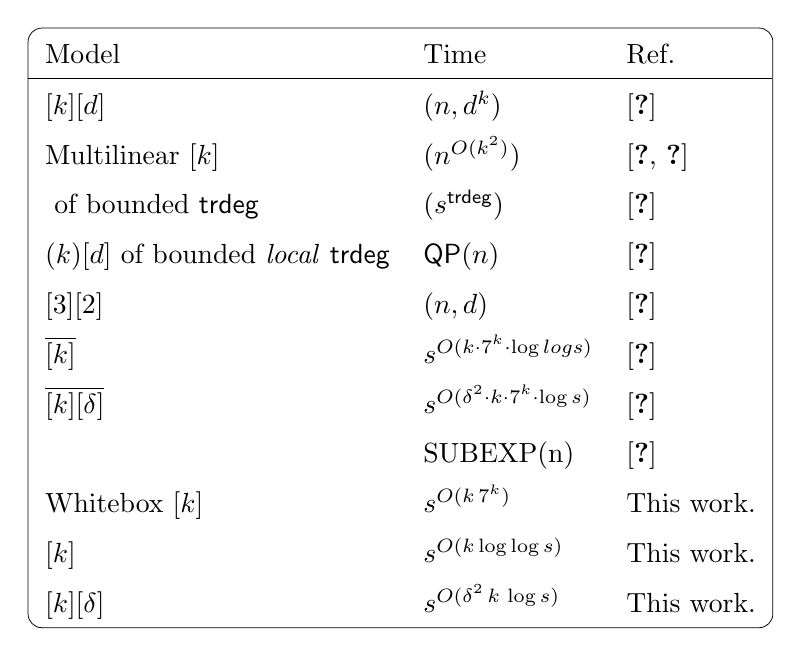
\begin{tikzpicture}[line width=.1mm,rounded corners=.5em]
        \node (table) [clip,inner sep=.5\pgflinewidth] {
        \begin{tabular}{llll}
%
            Model & Time & Ref. \\ \hline
            $\SPS{[k]}{[d]}$ & $\poly(n,d^k)$ & \cite{saxena2012blackbox} \\
            Multilinear $\SPSP{[k]}{}{}$ & $\poly(n^{O(k^2)})$ & \cite{saraf2018black,agrawal2016jacobian}\\
            $\SPSP{}{}{}$ of bounded $\mathsf{trdeg}$ & $\poly(s^{\mathsf{trdeg}})$ & \cite{beecken2013algebraic}\\ 
            $\SPSP{(k)}{}{[d]}$ of bounded \emph{local} $\mathsf{trdeg}$ & $\mathsf{QP}(n)$ & \cite{DBLP:journals/toc/0001S17} \\ 
            $\SPSP{[3]}{}{[2]}$ & $\poly(n,d)$ & \cite{peleg2020polynomial}\\
            $\overline{\SPSU{[k]}{}{}}$ & $s^{O(k \cdot 7^k \cdot \log log s)}$ & \cite{DDS21} \\
            $\overline{\SPSP{[k]}{}{[\delta]}}$ & $s^{O(\delta^2 \cdot k \cdot 7^k \cdot \log s)}$ & \cite{DDS21}\\
            $\SPSP{}{}{}$ & SUBEXP(n) & \cite{LST21}\\
            Whitebox $\SPSU{[k]}{}{}$ & $s^{O(k\,7^k)}$ & This work.\\
            $\SPSU{[k]}{}{}$ & $s^{O(k \log \log s)}$ & This work.\\
            $\SPSP{[k]}{}{[\delta]}$ & $s^{O(\delta^2\,k\,\log s)}$ & This work.\\
        \end{tabular}
        };
        \draw ([xshift=.5*\pgflinewidth,yshift=-.5*\pgflinewidth]table.north west) 
        rectangle ([xshift=-.5*\pgflinewidth,yshift=.5*\pgflinewidth]table.south east);
        \end{tikzpicture}
        \caption{Time complexity comparision of PIT algorithms related to $\SPSP{}{}{}$ circuits}
\end{table}

The authors recently generalised their novel $\DiDI$-technique to solve 'border PIT' of depth-4 circuits \cite{DDS21}. Specifically, they give a $s^{O(k \cdot 7^k \cdot \log log s)}$ time and $s^{O(\delta^2 \cdot k \cdot 7^k \cdot \log s)}$ time blackbox PIT algorithm for $\overline{\SPSU{[k]}{}{}}$ and $\overline{\SPSP{[k]}{}{[\delta]}}$ respectively. By definition, border classes capture exact complexity classes, hence border PIT results seemingly subsumes the results we present in this paper. However, the whitebox PIT algorithm here is much more efficient than their quasi-poly time blackbox algorithm. Further, the time complexity of blackbox PIT algorithms has a better dependence on $k$ and $\delta$ compared to their exponential dependence. Lastly, the proofs in this paper are simpler as we don't have to deal with an infinitesimally close approximation of polynomials in  border complexity classes. Very recently, Dutta and Saxena~\cite{duttaseparated21} showed an exponential-gap fanin-hierarchy theorem for bounded depth-3 circuits which is also based on a {\em finer} generalization of the $\DiDI$-technique.

In a breakthrought result by Limaye, Srinivasan and Tavenas \cite{LST21} the {\em first} superpolynomial lower bound for constant depth circuits was obtained. Their lower bound result, together with the `hardness vs randomness' tradeoff result of \cite{chou2018hardness} gives the {\em first} deterministic blackbox PIT algorithm for general depth-4 circuits which runs in $s^{O(n^\epsilon)}$ for all real $\epsilon > 0$. Their result is the first {\em sub}exponential time PIT algorithm for depth-4 circuits. Moreover, compared to their algorithm, our quasipoly time blackbox and polynomial time whitebox algorithms are significantly faster.

%
\medskip
{\bf Limitations of known techniques.}~~People have studied depth-$4$ PIT only with extra restrictions, mostly due to the limited applicability of the existing techniques as they were tailor-made for the specific models and do not generalize. E.g.~the previous methods handle  $\delta=1$ (i.e. linear polynomials at the bottom) or $k=2$ (via \emph{factoring}, \cite{saha2013case}). While $k=2$ to $3$, or $\delta=1$ to $2$ (i.e. `linear' to `quadratic') already demands a qualitatively different approach.  

Whitebox $\SPSU{[k]}{}{}$ model generalizes the famous bounded top fanin depth-$3$ circuits $\Sigma^{[k]}\Pi\Sigma$ of  \cite{kayal2007polynomial}; but their Chinese Remaindering (CR) method, loses applicability and thus fails to solve even a slightly more general model. The blackbox setting involved similar `certifying path' ideas in \cite{saxena2012blackbox} which could be thought of as general CR. It comes up with an ideal $I$ such that $f \ne 0 \bmod I$ and finally preserves it under a constant-variate linear map. The preservation gets harder (for both $\SPSU{[k]}{}{}$ and $\SPSP{[k]}{}{[\delta]}$) due to the increased non-linearity of the ideal $I$ generators. Intuitively, larger $\delta$ via ideal-based routes, brings us to the Gr\"obner basis method (which is doubly-exponential-time in $n$) \cite{vasconcelos2004computational}. We know that ideals even with $3$-generators (analogously $k=4$) already capture the whole ideal-membership problem \cite{sap19}.

The algebraic-geometric approach to tackle $\SPSP{[k]}{}{[\delta]}$ has been explored in \cite{beecken2013algebraic,gupta2014algebraic,mukhopadhyay2016depth,zeyu2021variety}. The families which satisfy a certain Sylvester–Gallai configuration (called SG-circuits) is the harder case which is conjectured to have constant transcendence degree \cite[Conj.~1]{gupta2014algebraic}. Non-SG circuits is the case where the nonzeroness-certifying-path question reduces to radical-ideal  non-membership questions \cite{garg2020special}. This is really a variety question where one could use algebraic-geometry tools to design a poly-time blackbox PIT. In fact, very recently, Guo \cite{zeyu2021variety} gave a $s^{\delta^k}$-time PIT by constructing explicit variety evasive subspace families. Unfortunately, this is not the case in the ideal non-membership; this scenario makes it much harder to solve $\SPSP{[k]}{}{[\delta]}$. From this viewpoint, radical-ideal-membership explains well why the intuitive $\Sigma^{[k]} \Pi \Sigma$ methods do not extend to  $\SPSP{[k]}{}{[\delta]}$.

Interestingly, Forbes \cite{forbes2015deterministic} found a quasipolynomial-time PIT for $\SWSP{}{}{[\delta]}$ using shifted-partial derivative techniques; but it naively fails when one replaces the $\wedge$-gate by $\Pi$ (because the `measure' becomes too large). The duality trick of \cite{saxena2008diagonal} completely solves whitebox PIT for $\SWSU{}{}$, by transforming it to a read-once oblivious ABP (ROABP); but it is inapplicable to our models with the top $\Pi$-gate (due to large waring rank and ROABP-width). A priori, our models are incomparable to ROABP, and thus the famous PIT algorithms for ROABP \cite{forbes2013quasipolynomial,forbes2014hitting,gurjarARO} are not expected to help either.

Similarly, a naive application of the \emph{Jacobian} and \emph{certifying path} technique from \cite{agrawal2016jacobian} fails for our models because it is difficult to come up with a \emph{faithful} map for constant-variate reduction. Kumar and Saraf \cite{DBLP:conf/coco/0001S16a} crucially used that the computed polynomial has low individual degree (such that~\cite{dvir2010hardness} can be invoked), while in \cite{DBLP:journals/toc/0001S17} they exploits the low algebraic rank of the polynomials computed below the top $\Pi$-gate. Neither of them hold in general for our models. Very recently, Peleg and Shpilka \cite{peleg2020polynomial} gave a poly-time blackbox PIT for $\SPSP{[3]}{}{[2]}$, via incidence geometry (e.g.~Edelstein-Kelly theorem involving `quadratic' polynomials), by solving \cite[Conj.~1]{gupta2014algebraic} for $k=3,\delta=2$. The method seems very strenuous to generalize even to `cubic' polynomials ($\delta=3=k$). 

\textbf{PIT for other models. } Blackbox PIT algorithms for many restricted models are known. Egs.~ROABP related models \cite{raz2005deterministic,jansen2010deterministic, agrawal2015hitting,gurjarARO,gurjar2017deterministic,forbes2014hitting,anderson2018identity}, $\log$-variate circuits \cite{forbes2018towards,bisht2020poly}, and non-commutative models \cite{garg2016deterministic,DBLP:journals/cjtcs/LagardeMP19}.

\subsection{Techniques and motivation}\label{sec:pf-ideas}

Both the proofs are analytic as they use \emph{logarithmic derivative}, and its power-series expansion which greatly transform the respective models. Where the nature of the first proof is inductive, the second is a more direct \emph{one-shot} proof. In both the cases, we essentially reduce to the well-understood \emph{wedge} models, that have unbounded top fanin, yet for which PITs are known. This reduction is unforeseeable and quite `power'ful.  

The analytic tool that we use, appears in algebra and complexity theory through the \emph{formal power series} ring $\ringR[[x_1,\hdots,x_n]]$ (in short $\ringR[[\x]]$), see \cite{10.2307/2317940,sinhababu2019power,dutta2018discovering}. The advantages of the ring $\ringR[[\x]]$ are many and they usually emerge because of the inverse identity: $(1 - x_1)^{-1} = \sum_{i \ge 0}\, x_1^i$, which does not make sense in $\ringR[x]$, but is valid in $\ringR[[\x]]$. Other analytic tools used are inspired from Wronskian (linear dependence) \cite[Theorem~7]{koiran2015wronskian} \cite{kayal2015lower}, Jacobian (algebraic dependence) \cite{beecken2013algebraic, agrawal2016jacobian,pandey2018algebraic}, and logarithmic derivative operator $\dlg_{\,z_1}(f) = (\partial_{z_1}\,f)/f$.

We will be work with the division operator (e.g.~ $\ringR(z_1)$, over a certain ring $\ringR$). However, the divisions do not come for free as they require invertibility with respect to $z_1$ throughout (again landing us in $\ringR[[z_1]]$. For circuit classes $C, D$ we define class \[\calC/\calD:=\{f/g \mid f\in \calC, \calD \ni g \neq 0\}.\]Similarly $\calC \cdot \calD$ to denotes the class taking respective products.

\subsubsection{The \texorpdfstring{$\DiDI$}{DiDI}-technique} In \autoref{thm:thm1} we introduce a novel technique for designing PIT algorithms which comprises of inductively applying two fundamental operations on the input circuits to reduce it to a more tractable model. Suppose we want to test $\sum_{i \in [k]} T_i \stackrel{?}{=} 0$ where each $T_i$ is computable by $\PSU{}{}$. The idea is to \emph{DI}vide it by $T_k$ to obtain $1 + \sum_{i \in [k-1]} T_i/T_k$ and then {\em D}erivative to reduce the fanin to $k-1$ and obtain $\sum_{i \in [k-1]} \calT_i$. Naturally, these operations pushes us to work with the fractional ring (e.g.~ $\ringR(z_1)$, over a certain ring $\ringR$), further it also distorts the model as $\calT_i$'s are no longer computable by simple $\PSU{}{}$ circuits. However, with careful analytically analysis we establish that the non-zeroness is preserved in the reduced model. The process is then repeated until we reach $k=1$, while maintaining the invariants which help us in preserving the non-zeroness till the end. We finish the proof by showing that the identity testing of reduced model can be done using known PIT algorithms.


\subsubsection{Jacobian hits again} In \autoref{thm:thm2} we exploit the prowess of the Jacobian polynomial first introduced in \cite{beecken2013algebraic} and later explored in \cite{agrawal2016jacobian} to unify known PIT algorithms and design new ones. Suppose we want to test $\sum_{i \in [k]} T_i \stackrel{?}{=} 0$, where $T_i \in \PSP{}{[\delta]}$ (respec.~$\PSU{}{}$). We associate the Jacobian $J(T_1, \hdots, T_r)$ to captures the algebraic independence of $T_1, \hdots, T_r$ assuming this to be a transcendence basis of the $T_i$’s. We design a variable reducing linear map $\Phi$ which preserves the algebraic independece of $T_1, \dots, T_r$ and show that for any $C$: $C(T_1,\hdots, T_k) = 0 \iff C(\Phi(T_1), \hdots, \Phi(T_k)) = 0$. Such a map is called `faithful' \cite{agrawal2016jacobian}. The map $\Phi$ ultimately provides a hitting set for $T_1 + \hdots +T_k$ , as we reduce to a PIT of a polynomial over `few' (roughly equal to $k$) variables, yielding a $\QP$-time algorithm.
